\section{Calculation of the energy level distance}
In the following task we should calculate the energy level distance of the absorption spectrum with two 
different methods. 
We limit the scan range again, instead of using the full scan range we will only 
be using the area from $140\,$mA to $160\,$mA. We determined that area because there is 
no visible mode jump in between. \\
\subsection{Current-Wavelength Relation}
As already done above, for this method we also use the current-wavelength relation figure \ref{fig:currentwave}.\\
After the wavelength and the current have been determined (Table: \ref{tab:laser current}), the energy level can be calculated for the four dips:
\begin{equation}
    E_i = h \cdot \nu = \frac{h c}{\lambda_i}
\end{equation}
In this formula c stands again for the speed of light and h stands for the Planck-constant. \\
The error of the energy is calculated as the following:
\begin{equation}
    s_{E_i} = \frac{hc}{\lambda_i^2} \cdot s_{\lambda}
\end{equation}
Here is the error of $\lambda$ the same as in the task before: $s_{\lambda}=0.0005\,$nm.\\
Next step is to calculate the energy level distance, therefore, we use the following equation:
\begin{equation}
    \Delta E = |E_i - E_{i+1}|
\end{equation}
With the formula mentioned above, the following values are obtained:
\begin{table}[h]
    \centering
        \begin{tabular}{c||c|c|c|c}
            Peak & $I$ in mA & $\lambda$ in nm & E in $10^{-24}\,$J & $\Delta E$ in $10^{-24}\,$J\\
            \hline
          1 & 142.2 & 780.2490 $\pm  0.0005$ & 254591.3 $\pm  0.2$ & 1.04 $\pm  0.23$\\
          2 & 147.3 & 780.2522 $\pm  0.0005$ & 254590.2 $\pm  0.2$ & 3.13 $\pm  0.23$\\
          3 & 153.6 & 780.2426 $\pm  0.0005$ & 254593.4 $\pm  0.2$ & 1.17 $\pm  0.23$\\
          4 & 156.2 & 780.2462 $\pm  0.0005$ & 254592.2 $\pm  0.2$ & \\
        \end{tabular}%
        \caption{Laser current, wavelength and frequency of the four peaks}
        \label{tab:A2data}%
    \end{table}\\
\subsection{Fabry-Perot-interferometer}
In this task we want to determine the energy level distance with a second method. This time we will using the Fabry-Perot-Interferometer (FPI). \\
Firstly, we need to calculate the free spectral range of the used FPI. 
\begin{equation}
    \Delta \nu_{FSR} = \frac{c }{2 \cdot n \cdot d} = \frac{c}{2 \cdot d} = 1.154200963 \cdot 10^8 Hz
\end{equation}
In the second equal sign was used that we have a refractive index of $n=1$ because the medium is air.
c is again the speed of light and d is the measured distance of the FPI, in our case its $d = c + d = 0.77\,$m.\\
Now we need to calculate the error of $\Delta \nu_{FSR}$, for this we use the error propagation:
\begin{align}
    s_{\Delta \nu_{FSR}} = \frac{\partial \Delta \nu_{FSR}}{\partial d} \cdot s_d = \frac{c}{2\cdot d^2} \cdot s_d = 758456.21 Hz
\end{align}
In the formula above the error of d is a read-off error  again and its value is: $s_d = 0.003\,$m. \\
With the preceding values follows for the free spectral range:
\begin{equation}
    \Delta \nu_{FSR} = (11.54 \pm 0.08) \cdot 10^7\,Hz
\end{equation}
In order to get the distances of the energy levels in the absorption spectrum you first have to count the number of dips $m$ from the figure:
\begin{figure}[h]
    \centering
    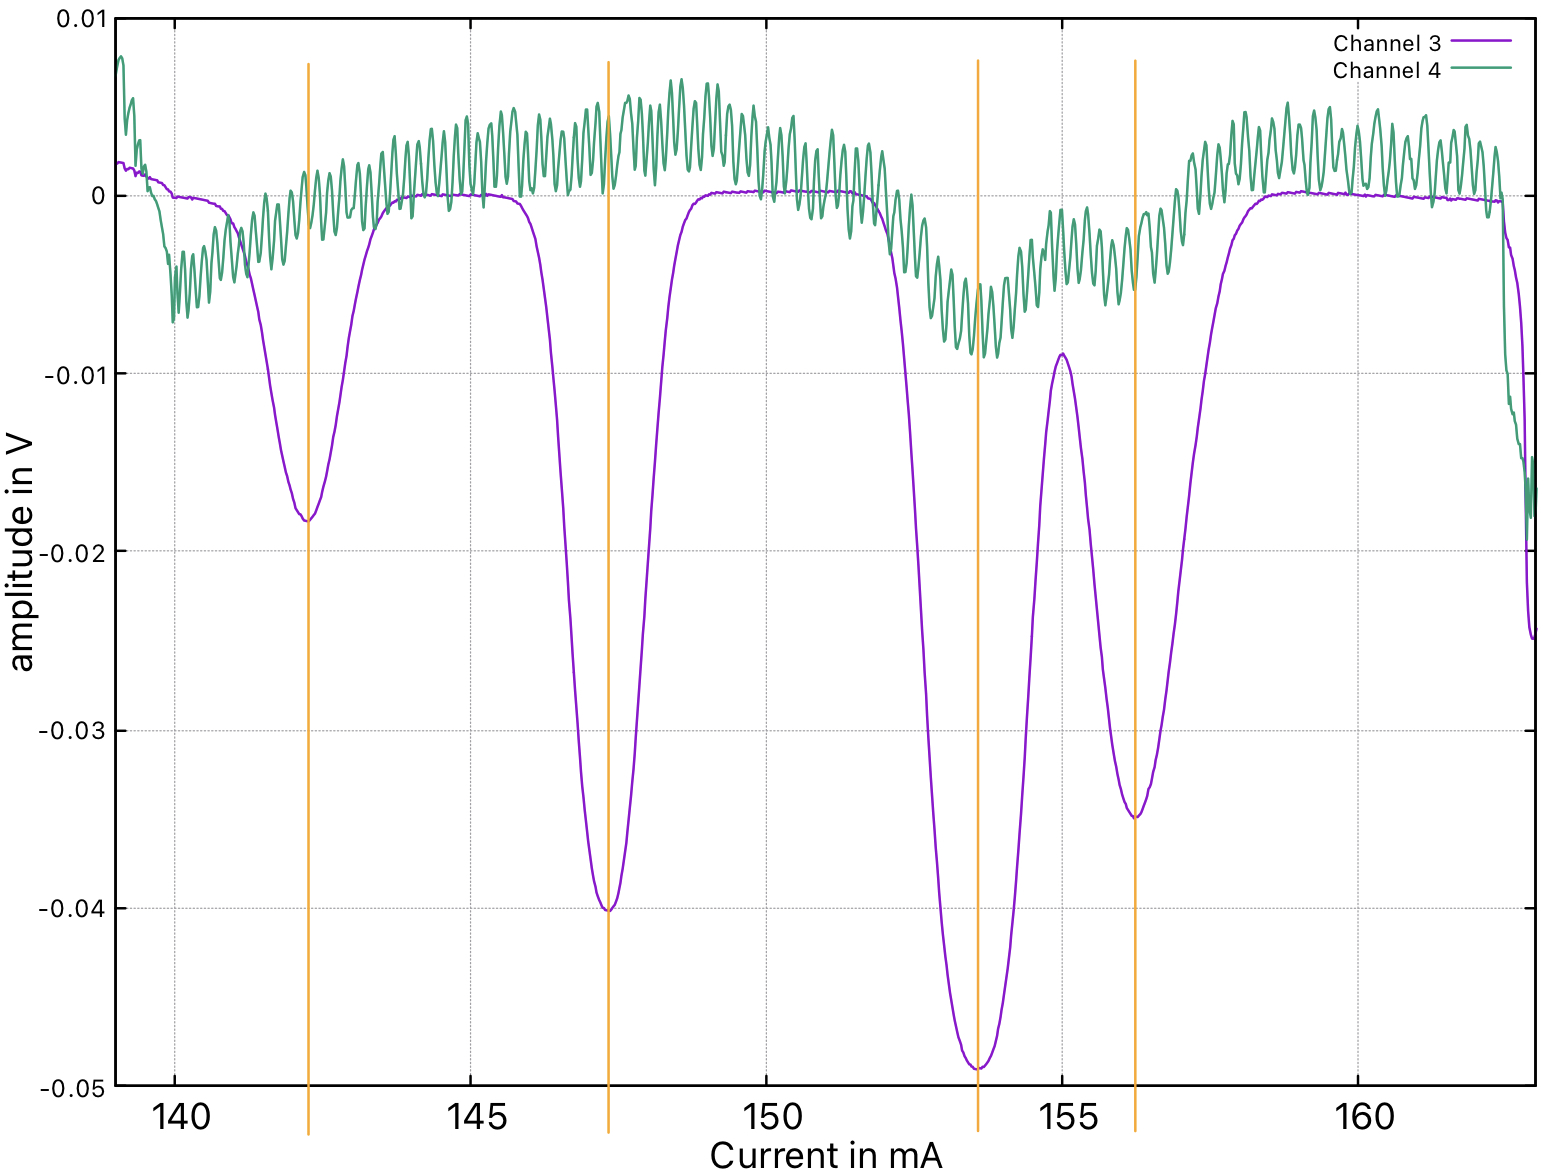
\includegraphics[scale = 0.2]{Bilder/Auswertung_Anna/A2-ver.jpg}
    \caption{trend free data with the drawn lines for the certain region.}
\end{figure}

However, only the dips in a certain region, i. e. between two different peaks, need to be considered.

Finally we get the energy level distance using the following equation:
\begin{equation}
    \Delta E = m \cdot h \cdot \Delta \nu_{FSR}
\end{equation}
Here is $m$ the number of the counted peaks in the specific area
and $h$ is again the Planck-constant.\\
Finally, we need to have a closer look at the error propagation of $\Delta E$.
\begin{equation}
    s_{\Delta E} = \sqrt{\Bigl(\frac{\partial \Delta E}{\partial m} \cdot s_m \Bigr) ^2 + \Bigl(\frac{\partial \Delta E}{\partial \Delta \nu_{FSR}} \cdot s_{\Delta \nu_{FSR}} \Bigr)^2 }
    = h \sqrt{(\Delta \nu_{FSR} \cdot s_m)^2+(m \cdot s_{\Delta \nu_{FSR}})^2}
\end{equation}
The error of $m$ is again a read-off error, because you have to read out the corresponding dips from a photo. As mentioned before it is not really accurate to read out of an photograph. 
\begin{table}[h]
    \centering
    \begin{tabular}{c||c|c}
        Distance & m& $\Delta E$ in $10^{-24}\,$ J \\
        \hline
          1-2 & 24 $\pm$ 1 & 1.828 $\pm  0.077$ \\
          2-3 & 29 $\pm$ 1 & 2.209 $\pm  0.077$ \\
          3-4 & 12 $\pm$ 2 & 0.914 $\pm  0.152$ \\
    \end{tabular}
        \caption{Distance of the energy level between two dips}
        \label{tab:A2second}
\end{table}
\begin{figure}[h]
    \centering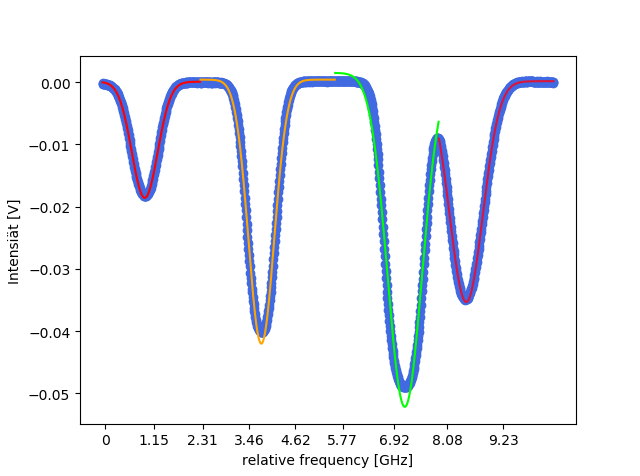
\includegraphics[width=0.8\textwidth]{Verbesserung/plot_all_gauss.png}
    \caption{Full plot of the data with relative frequency as x-axis}
\end{figure}
\subsection{Comparison of the two methods}
As you can see in the two tables \ref{tab:A2data} and \ref{tab:A2second} both methods lead to 
similar values if you only compare the order of magnitude. \\ 
Both methods are not really accurate. In both cases, the corresponding values had to be determined by means of pictures. 
However, the first method was even more inaccurate because one had to read out the wavelength with a second image. 
This significantly increases the uncertainty of this method. 
In the case of the second method, however, you also had to read the dips out of a graph and the area by which you have to count them. 
But due to the “zoomed in” area the difficulty is not too great to see the dips.
Nevertheless, this method is probably a bit more accurate because measured values such as the distance of the FPI were also used here.
